%----------------------------------------------------------------------------------------
%	PACKAGES AND THEMES
%----------------------------------------------------------------------------------------
\PassOptionsToPackage{table}{xcolor}
\documentclass[aspectratio=169,xcolor=dvipsnames,svgnames,x11names,fleqn]{beamer}
% \documentclass[aspectratio=169,xcolor=dvipsnames,fleqn]{beamer}

\usetheme{RedVelvet}

\usefonttheme[onlymath]{serif}
\newcommand{\showanswers}{yes}


\usepackage{xspace}
\usepackage{amsmath}
\usepackage{amssymb}
\usepackage{amsfonts}
\usepackage{color}
\usepackage{physics}
% \usepackage{mathbb}
\usepackage{rahul_math}
\usepackage{bigints}

\usepackage{graphicx} % Allows including images
\usepackage{booktabs} % Allows the use of \toprule, \midrule and \bottomrule in tables
\usepackage{tikz,pgfplots}

\usepackage{subfigure}
\usetikzlibrary{arrows}
\usepackage{minted}
\definecolor{LightGray}{gray}{0.9}
\definecolor{cream}{rgb}{0.92, 0.9, 0.55}
\definecolor{lightblue}{rgb}{0.68, 0.85, 0.9}


\usepackage{xcolor-material}
\usetikzlibrary{fit}
\usetikzlibrary{matrix}
\tikzset{%
apple/.pic={
  \fill [MaterialBrown] (-1/8,0)  arc (180:120:1 and 3/2) coordinate [pos=3/5] (@)-- ++(1/6,-1/7)  arc (120:180:5/4 and 3/2) -- cycle;
  \fill [MaterialLightGreen500] (0,-9/10)  .. controls ++(180:1/8) and ++(  0:1/4) .. (-1/3,  -1) .. controls ++(180:1/3) and ++(270:1/2) .. (  -1,   0) .. controls ++( 90:1/3) and ++(180:1/3) .. (-1/2, 3/4) .. controls ++(  0:1/8) and ++(135:1/8) .. (   0, 4/7)
}
}

\newcommand{\leftdoublequote}{\textcolor{blue}{\scalebox{3}{``}}}

\newcommand{\rightdoublequote}{\textcolor{blue}{\scalebox{3}{''}}}


\usepackage{textcomp}

\usepackage{overpic}

%----------------------------------------------------------------------------------------
%	TITLE PAGE
%----------------------------------------------------------------------------------------

\usepackage{tikz-qtree,tikz-qtree-compat}
\usetikzlibrary{calc}


\title[CPE 486/586: Machine Learning]{CPE 486/586: Machine Learning for Engineers} % The short title appears at the bottom of every slide, the full title is only on the title page
\subtitle{04 Statistics and Probability}

\author[Rahul Bhadani] {{\Large \textbf{Rahul Bhadani}}}

\institute[UAH] % Your institution as it will appear on the bottom of every slide, maybe shorthand to save space
{
    Electrical \& Computer Engineering,  The University of Alabama in Huntsville
}
\date

% \titlegraphic{
%    \includegraphics[width=0.4\linewidth]{figures/UAH_primary.png}
% }

\begin{document}

%-------------------------------------------------
\begin{frame}
    \titlepage
\end{frame}

%-------------------------------------------------
\begin{frame}{Outline}
    \backgroundtableofcontents
\end{frame}

\section{Probability}

\begin{frame}
    \sectionpage
\end{frame}





\begin{frame}[containsverbatim]{Probability Theory}
    \begin{enumerate}
        \item Probability is a branch of mathematics that deals with uncertainty.
        \item Probability is the likelihood or chance that something will occur. 
        \item Probability describes things whose outcomes are uncertain or random.
        
    \end{enumerate}
    \end{frame}
    
    %------------------------------------------------
    
    \begin{frame}[containsverbatim]{Sample Space}
    \begin{tblock}{Definition}
        A sample space $\Scal$ is the possible outcome of an experiment. A point $s$ in $\Scal$ is called sample outcome, realization, or outcome. Subsets of $\Scal$ are called events. 
        
        \textbf{Example: }
    
        In an experiment of tossing two coins, our sample space is $\Scal = \{HH, HT, TH, TT\}$. An event that at least one of the coins is heads is $\Ecal = \{HH, HT, TH\}$.
    \end{tblock}
    \end{frame}
    
    %------------------------------------------------
    
    \begin{frame}[containsverbatim]{Probability}
    \begin{tblock}{Definition}
       For each event $\Ecal$ in the sample space $\Scal$, the probability is a function which associates with $\Ecal$ a number between 0 and 1, i.e, $P(\Ecal) \in [ 0, 1]$.
    \end{tblock}
    \end{frame}
    
    %------------------------------------------------
    
    \begin{frame}[containsverbatim]{Probability}
        \begin{tblock}{Definition}
        It is technically hard to describe the probability of each single event. In that case, we consider a good collection $\Bcal$ of events which is large enough to contain all the useful events including $\emptyset$, and $\Scal$, and is closed under all possible countable set operations. This collection $\Bcal$ is called a sigma-algebra or Borel field. Probability is a set function defined only on this collection, i.e.,
        $$
        P: \Bcal \rightarrow [0, 1]
        $$
        
        \end{tblock}
    \end{frame}

    \begin{frame}{Probability: Example}

        \textbf{Example:} Tossing a fair die.
    
       \begin{enumerate}
           \item One possible $\sigma$-algebra $\Bcal_1$ is $\{ \emptyset, \Scal\}$.
           \item Another $\sigma$-algebra is the power set of $\Scal$.
           \item Another $\sigma$-algebra is $\Bcal = \{\emptyset, \Scal, \{0\}, \{2, 3, 4\}\}$.
       \end{enumerate}
        
    \end{frame}
    
    %------------------------------------------------
    
    \begin{frame}[containsverbatim]{Conditional Probability}
        \begin{tblock}{Definition}
            The probability of an event A given B is defined as
            \begin{equation}
                P(A|B) = \cfrac{P(A \cap B )}{P(B)}
            \end{equation}
            given $P(B) > 0$.
        \end{tblock}
    \end{frame}

    \begin{frame}[containsverbatim]{Conditional Probability}
        \begin{facts}{Some facts}
            \begin{enumerate}
                \item $P(B|B) = 1$
                \item $P(A|B) = \cfrac{P(A)}{P(B)} \text{~for~} A \subset B$
                \item $P (B|A) = 1  \text{~for~}  A \subset B$
                \item  Multiplication formula is useful when it is easier to obtain conditional probability: $P(A\cap B) = P(B) P(A|B)  = P(A) P(B|A)$.
                \item $P(A) = P(A\cap B)+ P(A \cap B^c) = P(B)P(A|B) + P(B^c) P(A|B^c)$ , where $B^c$ is the complement of $B$.
            \end{enumerate}
        \end{facts}
    \end{frame}
    \begin{frame}[containsverbatim]{Conditional Probability}

        \begin{exampleblock}{Example 1}
            Let box 1 contain 2 red balls and 3 green balls and box 2 contain 5 red balls and 4 green balls. One box is chosen at random and one ball is drawn randomly from the chosen box. What is the probability of getting a red ball?
        \end{exampleblock}
    \end{frame}
    \begin{frame}[containsverbatim]{Conditional Probability}
        \ifthenelse{\equal{\showanswers}{yes}}
        {
        \begin{examplesolution}{Example 1 Solution}
            
            Consider event A  = choosing a red ball, even B = choosing the first box. Then $P(B) = P(B^c) = \cfrac{1}{2}$ ($B^c$ is the complement of $B$).
            Then, the probability of drawing a red ball given the first box can be written as  $P(A|B) = \cfrac{2}{5}$.
            $P(A|B^c) = \cfrac{5}{9}$.
            Then the probability of getting a red ball is $P(A) = \cfrac{1}{2}\times\cfrac{2}{5} + \cfrac{1}{2}\times\cfrac{5}{9}  = \cfrac{43}{90}$.
        \end{examplesolution}
        }{
            \textbf{Solution:} \color{LightGray}{Blank space for calculation}
        }
    \end{frame}
    
    %------------------------------------------------
    
    \begin{frame}[containsverbatim]{Bayes' Rule as Inversion of Conditional Probability}
    
    Assume that we can partition sample space $\Scal$ into $B_1, B_2, B_3$. The conditional probabilities can be $P(A|B_i), i = 1, 2, \cdots.$ Then, the posterior probabilities can be written as 
    \begin{equation}
        P(B_i | A) = \cfrac{P(B_i \cap A)}{P(A)} = \cfrac{P(B_i)P(A|B_i)}{\sum_j P(B_j)P(A|B_j)}
    \end{equation}

\end{frame}

\begin{frame}[containsverbatim]{Bayes' Rule as Inversion of Conditional Probability}
    
    \begin{exampleblock}{Example 1 Extension}
        Consider the example 1 from the previous section. Given that we obtained a red ball, what is the probability that box 1 was selected?
    \end{exampleblock}
    
\end{frame}

\begin{frame}[containsverbatim]{Bayes' Rule as Inversion of Conditional Probability}
    \ifthenelse{\equal{\showanswers}{yes}}
{
    \begin{examplesolution}{Example 1 Extension Solution}
        We are interested in determining $P(B|A)$. From the Bayes' Rule, 
    
        \begin{equation}
            P(B|A) = \cfrac{\frac{1}{2}\times \frac{2}{5}}{\frac{1}{2}\times \frac{2}{5} + \frac{1}{2}\times \frac{5}{9}} = \cfrac{\cfrac{1}{5}}{\cfrac{43}{90}} = \cfrac{18}{43}
        \end{equation}
    \end{examplesolution}
}{
    \textbf{Solution:} \color{LightGray}{Blank space for calculation}
}
\end{frame}

\begin{frame}[containsverbatim]{Bayes' Rule as Inversion of Conditional Probability}
    
    \begin{exampleblock}{Example 2: Rare disease probability}
        Consider that the probability of occurrence of a disease is 1/1000. A test accurately predicts the occurrence with 99\% accuracy and negates the disease with 98\% accuracy. Given that the test has shown positive, what is the probability of actually having the disease?
    \end{exampleblock}
    
\end{frame}

\begin{frame}[containsverbatim]{Bayes' Rule as Inversion of Conditional Probability}
    \ifthenelse{\equal{\showanswers}{yes}}
    {
    \begin{examplesolution}{Example 2 Solution: Rare disease probability}
        Let's consider $B_1$ = event of the occurrence of disease, $B_2 = $ event that the patient is healthy.
        $A$ = event that a patient has been tested positive.
    
        From the question, we have $P(B_1) = 0.001$.
        $P(B_2) = 1  - P(B_1) = 0.999$
    
        $P(A|B_1) = 0.99$, $P(A|B_2) = 0.02$, then fron Bayes' rule
    
        \begin{equation}
            P(B_1 | A) = \cfrac{0.001 \times 0.99}{0.001 \times 0.99 + 0.999\times 0.02} = 0.047210
        \end{equation}
    \end{examplesolution}    
    }{
        \textbf{Solution:} \color{LightGray}{Blank space for calculation}
    }
    \end{frame}
    
    %------------------------------------------------
    
    \begin{frame}[containsverbatim]{Independence}
        \begin{tblock}{Definition}
            Two events are independent if the occurrence of one of the events gives us no information about whether or not the other event will occur. In other words, events do not influence each other. Formally, we write
    
            \begin{equation}
                P(A|B) = P(A)
            \end{equation}
            which is still applicable even if $P(A)$ or $P(B)$ is 0.
        \end{tblock}

    \end{frame}
    
    %------------------------------------------------
    
    \begin{frame}[containsverbatim]{Independence}
    
        $P(A|B) = P(A)$ is equivalent to $P(A \cap B) =  P(A)P(B)$, that is, the probability that they both occur is equal to the product of the probabilities of the two individual events.

    \end{frame}
    
    %------------------------------------------------
    
    \begin{frame}[containsverbatim]{Independence: Symmetric Relationship and Unrelated Events}
        \large
        \begin{center}
            Symmetric relationship: A is independent of B implies B is independent of A.

            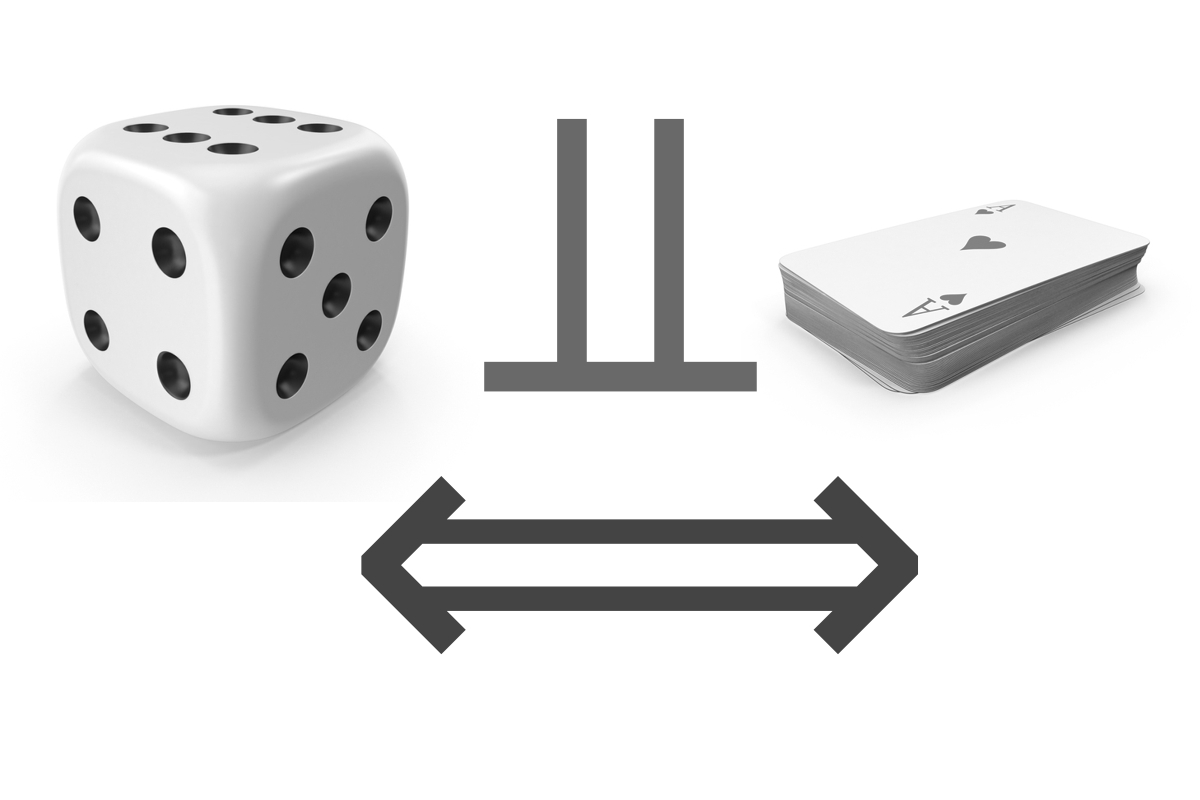
\includegraphics[width=0.4\linewidth]{figures/dice_cards.jpg}

            Unrelated events must be independent.
        \end{center}
    \end{frame}
    
    
    \begin{frame}[containsverbatim]{Independence vs. Mutual Exclusivity}
       
        \begin{center}
            Independent and mutually exclusive events are not the same. If $P(A) > 0$, and $P(B) > 0$, then:
            \begin{enumerate}
                \item If $A$ and $B$ are mutually exclusive, they cannot be independent.
                \item If $A$ and $B$ are independent, they cannot be mutually exclusive.
            \end{enumerate}

            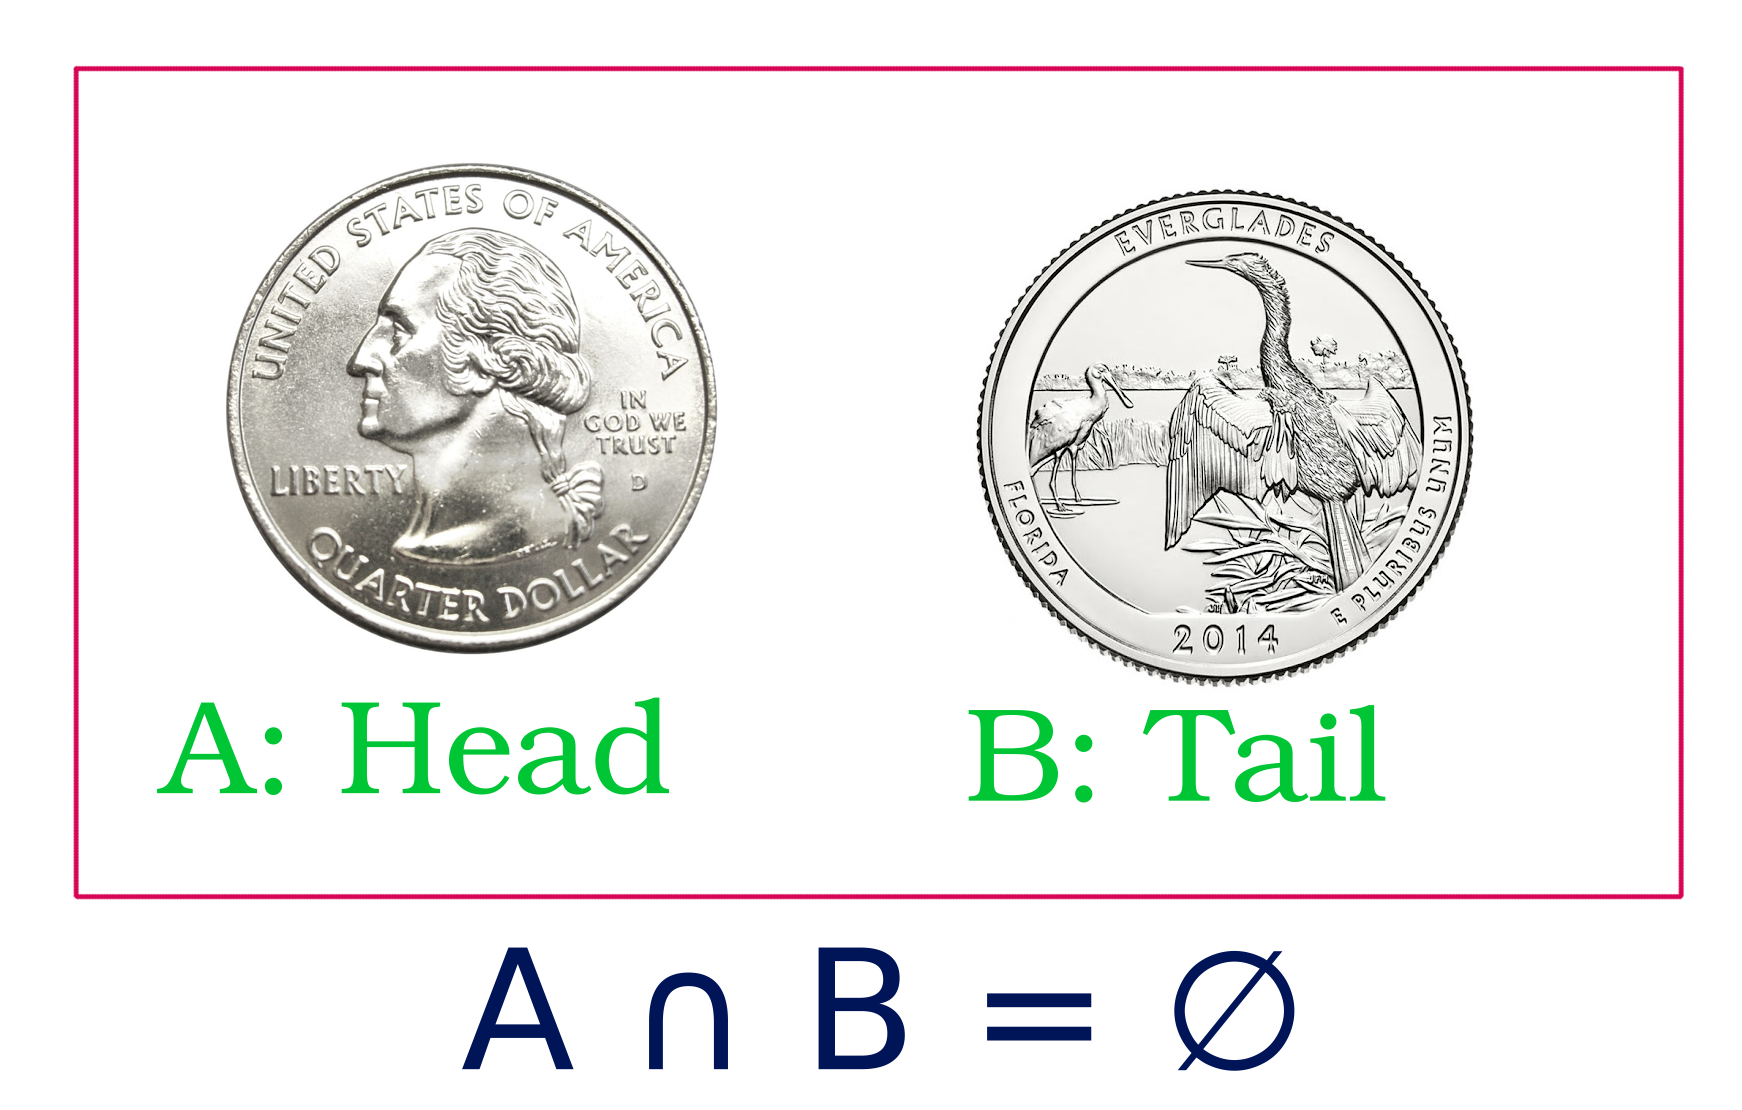
\includegraphics[width=0.4\linewidth]{figures/mutual_exclusive.png}

                \textbf{Mutually exclusive but not independent}
        
            \end{center}
    \end{frame}
    
    \begin{frame}[containsverbatim]{Independence: Complementary Events}
        \Large
        If $A$ and $B$ are independent, so are $A, B^c$ ; $A^c, B$; and $A^c, B^c$.
        
    \end{frame}
    
    \begin{frame}[containsverbatim]{Independence of Multiple Events}
        The idea of independence can be extended to more than two events. For example, $A$, $B$, and $C$ are independent if:
            \begin{enumerate}
                \item $A$ and $B$ are independent,
                \item $A$ and $C$ are independent, and  
                \item $B$ and $C$ are independent; and 
                \item $P(A \cap B \cap C) = P(A)P(B)P(C)$.
            \end{enumerate}
      
    \end{frame}
    
    
    %------------------------------------------------
    
    \begin{frame}[containsverbatim]{Independence}

        \begin{exampleblock}{Example 3}
            Let's say that a man and a woman each have a pack of 52 playing cards. Each draws a card from his/her pack. Find the probability that they each draw the ace of clubs $\clubsuit$.
        \end{exampleblock}
        \begin{center}
            
\includegraphics[width=0.3\linewidth]{figures/deck_of_cards.jpg}
        \end{center}
        \end{frame}
    
    %------------------------------------------------
    
    \begin{frame}[containsverbatim]{Independence}
    
        \ifthenelse{\equal{\showanswers}{yes}}
        {
        \begin{examplesolution}{Example 3 Solution}
           As they are drawing their cards independently of each other, the required probability is $\cfrac{1}{52} \times \cfrac{1}{52}$.
        \end{examplesolution}
        }
        {
            \textbf{Solution:} \color{LightGray}{Blank space for calculation}
        }
    \end{frame}
    
    %------------------------------------------------
    
    \begin{frame}[containsverbatim]{Independence}
    
        \begin{exampleblock}{Example 4}
        What is the chance of getting at least one six in 4 throws of a dice?
        \end{exampleblock}

        \begin{center}
            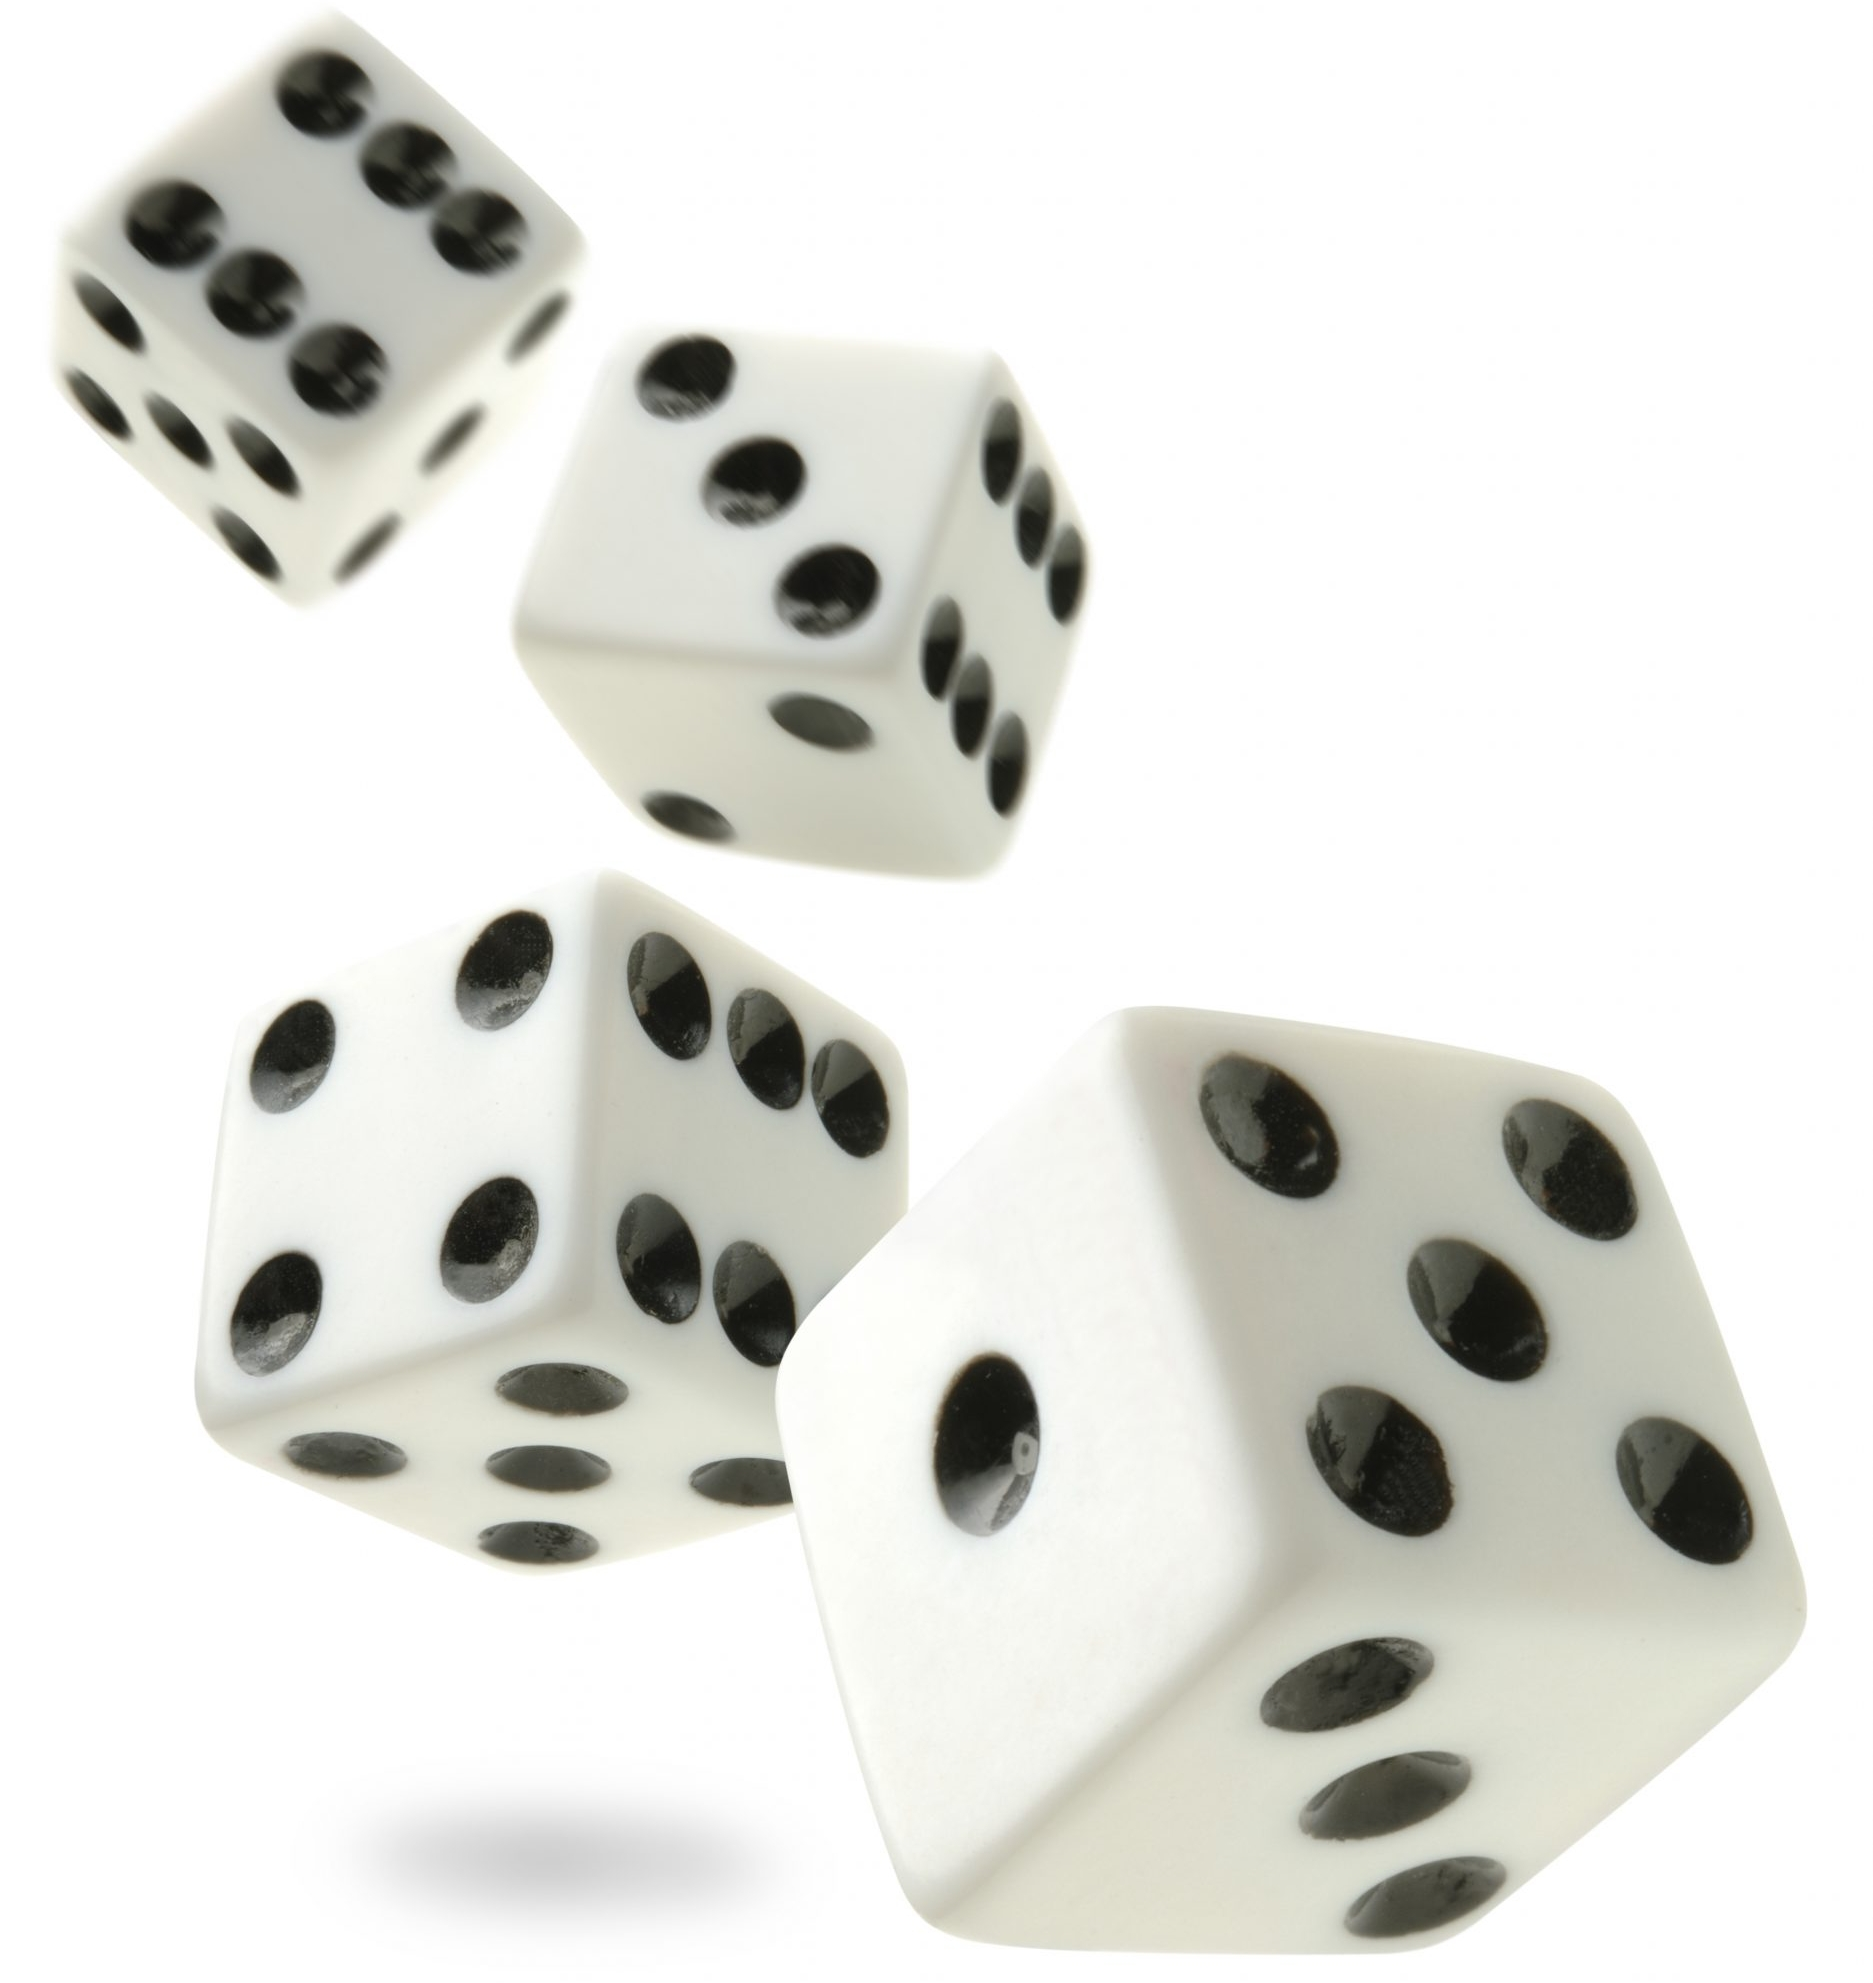
\includegraphics[width=0.15\linewidth]{figures/four_dice.jpg}
        \end{center}

    \end{frame}
    
    %------------------------------------------------
    
    \begin{frame}[containsverbatim]{Independence}
        \ifthenelse{\equal{\showanswers}{yes}}
        {
    \begin{examplesolution}{Example 4 Solution}
        We first calculate the probability of no six in 4 throws of a dice which is given by $(5/6)^4$ as each throw is independent of one another. Thus the probability of getting at least one six in 4 throws of a dice is $1 - (5/6)^4$.
        \end{examplesolution}
        }
        {
            \textbf{Solution:} \color{LightGray}{Blank space for calculation}
        }
    \end{frame}

\section{Statistics}

\begin{frame}
    \sectionpage
\end{frame}


    %%%%%%%%%%%%%%%%%%%%%%%%%%%%%%%%%%%%%%%%%%%%%%%%%%%%%

\subsection{Random Variable}

\begin{frame}
    \subsectionpage
\end{frame}


\begin{frame}[containsverbatim]{Random Variable}
    \begin{tblock}{Definition}
        A random variable is a real-valued function defined on the sample space $\Scal$, that is a rule which assigns a number to each outcome. Random variables can be thought of as a stochastic function. Random variables are denoted by capital letters such as $X, Y, Z$. The outcome of random variables is represented with corresponding small letters such as $x, y, z$.
    
    \end{tblock}

\end{frame}



\begin{frame}[containsverbatim]{Random Variable}
    \begin{tblock}{Example}

        {\color{blue}{For example, the probability that a random variable takes the value of 2 would be expressed as $P(X = 2)$ where $x = 2$.}}
    
        
        \begin{itemize}
            \item[-] A random variable is a function $\Scal \to \Rbb$.
        \end{itemize}
    
    $\bullet$ A random variable is called discrete if it takes only a finite or countably many values.\newline
    $\bullet$ A random variable is called continuous if it can assume all the values in an interval.
    \end{tblock}
    
\end{frame}

\begin{frame}[containsverbatim]{Probability Mass Function}
    
    \begin{gradblock}{Definition}
        At this point, we can transition from probability to probability law which will help us in writing computer programs at a later stage.
    
        The probability law of a discrete random variable can be described by the function defined as 
        \begin{equation}
            p(x) = P(X = x)
        \end{equation}
    \end{gradblock}

\end{frame}

\begin{frame}[containsverbatim]{Probability Mass Function}
    
    
    Let $x_1, x_2, \cdots $ be the points where $p$ gives positive masses (or values) that we can call $p_1, p_2, \cdots$. Thus $P(X = x_j) = p_j, j = 1, 2, \cdots $
    \begin{itemize}
        \item $p_j \geq 0$, and $\sum_{j= 1}^\infty p_j = 1$.
    \end{itemize}

\end{frame}

\begin{frame}[containsverbatim]{Probability Mass Function: Example}
    
    
    \begin{exampleblock}{Example 5}
    If a coin is tossed twice, the sample space $\Scal = \{HH, HT, TH, TT\}$. Let $X$ be the random variable that denotes the number of heads that can come up. With each sample point, we can associate a number for X, as shown below:
    
    \begin{tabular}{|c|c|c|c|c|}
    \hline
     & \textbf{HH} & \textbf{HT} & \textbf{TH} & \textbf{TT} \\
    \hline
    \textbf{X} & 2 & 1 & 1 & 0 \\
    \hline
    \end{tabular}
    \newline
    \newline
    \textbf{Note:} We can also define some other random variable on the same sample space, such as the square of the number of heads, i.e. $Y = X^2$ or the number heads minus the number of tails $Z = X - W$, where $W$ is the random variable the denotes the number of tails that can come up.
    \end{exampleblock}

\end{frame}

\begin{frame}[containsverbatim]{Probability Mass Function: Example}
    
    
    \begin{exampleblock}{Example 6}
        \begin{equation}
            p_k = P(X = k) = q^{k-1} p, \text{~where~} 0 < p < 1 , q = 1 - p, \quad k = 1, 2, \cdots
        \end{equation}
        This is pmf as it satisfies $p_k \geq 0$, and $\sum_{k=0}^\infty p_k = 1.$
    \end{exampleblock}

\end{frame}

\begin{frame}[containsverbatim]{Probability Density Function}
    
    
    When it comes to the continuous random variable $X$ that takes real values, then it is not possible to define the probability for a single point, as they are real values. {\color{red}{At what real value we should define a probability -- there can be a possibility of an infinite number after a decimal point!!!}. }
    Hence, we definite the probability over a range. In this case, we get the probability density function (PDF) $p(x)$ such that 
    \begin{equation}
        P(x_0 < x < x_1) = \int_{x_0}^{x_1} p(x)dx.
    \end{equation}

\end{frame}

\begin{frame}[containsverbatim]{Probability Density Function}
    
    

    Endpoints ${x_0}$ and ${x_1}$ may not be included. They do not matter for continuous random variable $X$. In this case, $p(x)$ satisfies the following property:
    \begin{itemize}
        \item $p(x) \geq 0 \quad \forall x$
        \item $\int_{-\infty}^\infty p(x) dx = 1$
    \end{itemize}
  

    \end{frame}
    
        %%%%%%%%%%%%%%%%%%%%%%%%%%%%%%%%%%%%%%%%%%%%%%%%%%%%%

\subsection{Probability Distribution}
\begin{frame}
    \subsectionpage
\end{frame}

    
    \begin{frame}[containsverbatim]{Cumulative Distribution Function (CDF)}
    
    \begin{tblock}{Definition}
        For any $x\in \Rbb$, we define cumulative distribution function as 
    
        \begin{equation}
            F(x) = P(X\leq x)
        \end{equation}
    They are sometimes to referred just as \textbf{distribution} or \textbf{probability distribution}. Shorthand notation for CDF is $F_X$.
    \end{tblock}

\end{frame}
\begin{frame}[containsverbatim]{CDF:Example}
   

    \begin{exampleblock}{Example 7: CDF of a Discrete Random Variable}
        Consider a discrete random variable $X$ such that $P(X = 0) = 1/3$, $P(X = 1) = 1/2$, $P(X =2) 1/6$. Then pmf of $X$, $p(x)$ is written as $p(0)= 1/3$, $p(1) = 1/2$, $p(2) = 1/6$ and $p(x) = 0$ for all other $x$.
    
        The CDF of $X$, $F(X)$ is given by 
        \begin{equation}
            F(x) = \begin{cases}
                0, \quad x< 0\\
                1/3, \quad 0\leq x \leq 1\\
                5/6, \quad 1\leq x < 2\\
                1, \quad x\geq 2
            \end{cases}
        \end{equation}
    In this case, the graph of F is a step function, having jumps at the point where $X$  has mass.
    \end{exampleblock}

\end{frame}
\begin{frame}[containsverbatim]{CDF: Example}
    
    What would be the CDF from Example 6?

    \ifthenelse{\equal{\showanswers}{yes}}
        {
            \begin{multiequation}
                F(x) & = P(X \leq k)\\
                & = q^0 +  q^1 p + q^2 p + \cdots + q^{k-1} p\\
                & = p( q^0 + q^1 + q^2 + \cdots + q^{k-1})
            \end{multiequation}
            We apply geometric progression formula $S_{GP} = \cfrac{a(1-r^n)}{1-r}$ where $a$ is the first term in GP and $r$ is the common ratio. Hence,
            \begin{multiequation}
                F(x) = p \cfrac{q^k -1}{q-1}
            \end{multiequation}
        }
        {
            \textbf{Solution:} \color{LightGray}{Blank space for calculation}
        }

\end{frame}
\begin{frame}[containsverbatim]{CDF of a Continuous Random Variable (RV)}
    
    
  
    For a continuous RV, we can define the CDF as 
    \begin{equation}
        F(x) = \int_{-\infty}^{x} f(t)dt 
    \end{equation}
    for the probability density function (PDF) $f(x)$. We also write $f_X$ to denote that $f$ is the PDF of the random variable $X$.
    Here, $t$ is the dummy variable of the integration. 
    \begin{enumerate}
        \item If $F(x)$ is differentiable at a given point, then $f(x) = F'(x)$.
        \item $f$ must satisfy
        \begin{equation}
            f(t) \geq 0, \quad \int_{-\infty}^\infty f(t)dt = 1.
        \end{equation}
    \end{enumerate}
    
\end{frame}
\begin{frame}[containsverbatim]{Identically Distributed}
    


        If $X$ and $Y$ are two random variables with $P(X \in A) = P(X \in A)$ for all sets $A$. Then, they are called identically distributed. This is equivalent to $F_X(x) = F_Y(x)$ for all $x$, i.e. two CDFs are equal.
    \end{frame}
    \begin{frame}[containsverbatim]{Independent and Identically Distributed (IID)}
        
        In addition to identically distributed, if two random variables are mutually independent, then they are called independent and identically distributed or (IID). It means sample items are independent events; the knowledge of the value of one variable will not give any information about the value of the other and vice versa.
 
    \end{frame}

    \begin{frame}[containsverbatim]{Example}
        

    \begin{exampleblock}{Example 8}
        Hit a dartboard of radius $R$ randomly. Let $X$ be the random variable denoting the distance of the chosen point from the center. In this case, probabilities are proportional to area, so $F(x) = P(X\leq x) = \cfrac{\pi x^2}{\pi R^2} = (x/R)^2, \quad 0 \leq x \leq R$. 
    \end{exampleblock}
    \end{frame}
    
    %------------------------------------------------
    \begin{frame}{Expected Values or Expectations}
        Consider a random variable $X$ with pdf or pmf $f(x)$.
        If we have a function $g(X)$ of a random variable, then we can define the expectation as 
        \begin{equation}
            \Ebb( g(X)) = \begin{cases}
                \int_{-\infty}^\infty g(x) f(x) dx, \quad \text{~if~} X \text{~is continuous}\\
                \sum_{x\in \Xcal} g(x) f(x), \quad \text{~if~} X \text{~is discrete}
            \end{cases}
        \end{equation}
    provided that $|\Ebb(g(X)| < \infty$. If $|\Ebb(g(X)| = \infty$, we say that the expectation doesn't exist. Here $\Xcal$ is the sample space of the random variable $X$.
    
    Some literature also write $E$ instead of $\Ebb$ for the expectation.
    
    {\color{red}{Expectation is also referred to as mean or average.}}
    \end{frame}
    
    %------------------------------------------------
    \begin{frame}{Median}
        If $X$ is a continuous random variable and has CDF $F_X$. Its median $m$ is the value that satisfies $F_X(m) = 1/2$, that is,
        \begin{equation}
            \int_{-\infty}^m f_X(x) dx = \int_m^\infty f_X(x)dx = \cfrac{1}{2}
        \end{equation}
        Equivalently, $m = F^{-1}_X (1/2)$.
    \end{frame}
    
    %------------------------------------------------
    \begin{frame}{Variance and Standard Deviation}
    The variance of a random variable $X$ can be defined as 
    \begin{equation}
        var(X) = \Ebb(X - \Ebb(X))^2
    \end{equation}
    We also denote $\sigma^2 = var(X)$. The standard deviation of $X$ is the square root of $var(X)$,i.e.,
    \begin{equation}
        \sigma = \sqrt{var(X)}
    \end{equation}
    Variance and standard deviation measure the degree of spread of a distribution around its mean $\Ebb(X)$.
    \end{frame}


    \subsection{Statistical Moments}

        
    \begin{frame}
    \subsectionpage
    \end{frame}

    \begin{frame}{Statistical Moments}
        \footnotesize

\begin{itemize}
    \item Statistical moments describe the shape and characteristics of probability distributions
    \item The $k$-th moment about the origin is defined as:
    $$\mu_k' = E[X^k] = \int_{-\infty}^{\infty} x^k f(x) dx$$
    \item The $k$-th central moment is:
    $$\mu_k = E[(X - \mu)^k] = \int_{-\infty}^{\infty} (x - \mu)^k f(x) dx$$
    \item First four moments provide crucial distribution information:
    \begin{itemize}
        \item $\mu_1' = \mu$ (mean) $ =  \mu = \frac{\sum_{i=1}^{N} x_i}{N} $
        \item $\mu_2 = \sigma^2$ (population variance)  $ = \frac{\sum_{i=1}^{N}(x_i - \mu)^2}{N}$\\
        
        Sample Variance: $s^2 = \frac{\sum_{i=1}^{n}(x_i - \bar{x})^2}{n-1}$

        \item $\mu_3$ relates to skewness
        \item $\mu_4$ relates to kurtosis
    \end{itemize}
\end{itemize}
\end{frame}

\begin{frame}{Skewness: Measuring Asymmetry}
\begin{block}{Definition}
Skewness measures the asymmetry of a probability distribution around its mean.
\end{block}

\begin{itemize}
    \item \textbf{Population Skewness:}
    $$\gamma_1 = \frac{\mu_3}{\sigma^3} = \frac{E[(X - \mu)^3]}{\sigma^3}$$
    
    \item \textbf{Sample Skewness (Pearson's moment coefficient):}
    $$g_1 = \frac{m_3}{s^3} = \frac{\frac{1}{n}\sum_{i=1}^{n}(x_i - \bar{x})^3}{s^3}$$
    
    \item \textbf{Adjusted Sample Skewness:}
    $$G_1 = \frac{\sqrt{n(n-1)}}{n-2} \cdot g_1$$
\end{itemize}
\end{frame}
s

% Frame 3: Interpreting Skewness
\begin{frame}{Interpreting Skewness Values}
\begin{columns}
\begin{column}{0.5\textwidth}
\begin{itemize}
    \item $\gamma_1 = 0$: Perfectly symmetric
    \item $\gamma_1 > 0$: Right-skewed (positive skew)
    \item $\gamma_1 < 0$: Left-skewed (negative skew)
\end{itemize}

\vspace{0.5cm}
\textbf{Rule of thumb:}
\begin{itemize}
    \item $|\gamma_1| < 0.5$: Approximately symmetric
    \item $0.5 \leq |\gamma_1| < 1$: Moderately skewed
    \item $|\gamma_1| \geq 1$: Highly skewed
\end{itemize}
\end{column}

\begin{column}{0.5\textwidth}
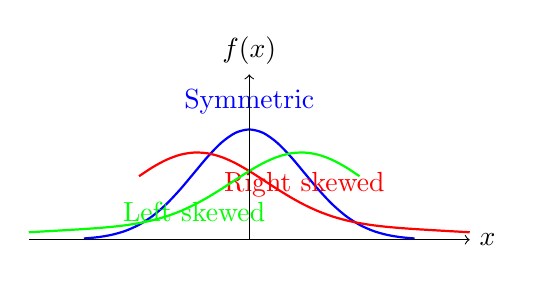
\begin{tikzpicture}[scale=0.7]
% Normal distribution
\draw[thick, blue] plot[smooth, domain=-3:3] (\x, {2*exp(-0.5*\x*\x)});
\node[blue] at (0, 2.5) {Symmetric};

% Right skewed
\draw[thick, red] plot[smooth, domain=-2:4] (\x, {1.5*exp(-0.3*(\x+1)*(\x+1)) + 0.2*exp(-0.1*(\x-2)*(\x-2))});
\node[red] at (1, 1) {Right skewed};

% Left skewed
\draw[thick, green] plot[smooth, domain=-4:2] (\x, {0.2*exp(-0.1*(\x+2)*(\x+2)) + 1.5*exp(-0.3*(\x-1)*(\x-1))});
\node[green] at (-1, 0.5) {Left skewed};

\draw[->] (-4,0) -- (4,0) node[right] {$x$};
\draw[->] (0,0) -- (0,3) node[above] {$f(x)$};
\end{tikzpicture}
\end{column}
\end{columns}
\end{frame}

% Frame 4: Kurtosis Definition
\begin{frame}{Kurtosis: Measuring Tail Behavior}
\begin{block}{Definition}
Kurtosis measures the "tailedness" and peakedness of a probability distribution.
\end{block}

\begin{itemize}
    \item \textbf{Population Kurtosis:}
    $$\gamma_2 = \frac{\mu_4}{\sigma^4} = \frac{E[(X - \mu)^4]}{\sigma^4}$$
    
    \item \textbf{Sample Kurtosis:}
    $$g_2 = \frac{m_4}{s^4} = \frac{\frac{1}{n}\sum_{i=1}^{n}(x_i - \bar{x})^4}{s^4}$$
    
    \item \textbf{Excess Kurtosis:}
    $$\text{Excess Kurtosis} = \gamma_2 - 3$$
    (Normal distribution has kurtosis = 3, so excess kurtosis = 0)
\end{itemize}
\end{frame}

% Frame 5: Types of Kurtosis
\begin{frame}{Types of Kurtosis}
\begin{columns}
\begin{column}{0.5\textwidth}
\begin{itemize}
    \item \textbf{Mesokurtic:} $\gamma_2 = 3$ (Normal distribution)
    \item \textbf{Leptokurtic:} $\gamma_2 > 3$ (Heavy tails, sharp peak)
    \item \textbf{Platykurtic:} $\gamma_2 < 3$ (Light tails, flat peak)
\end{itemize}

\vspace{0.5cm}
\textbf{Excess Kurtosis Interpretation:}
\begin{itemize}
    \item Excess $= 0$: Normal-like tails
    \item Excess $> 0$: Heavier tails than normal
    \item Excess $< 0$: Lighter tails than normal
\end{itemize}
\end{column}

\begin{column}{0.5\textwidth}
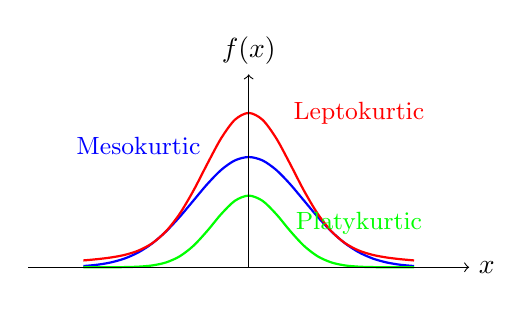
\begin{tikzpicture}[scale=0.7]
% Normal (mesokurtic)
\draw[thick, blue] plot[smooth, domain=-3:3] (\x, {2*exp(-0.5*\x*\x)});
\node[blue] at (-2, 2.2) {\small Mesokurtic};

% Leptokurtic
\draw[thick, red] plot[smooth, domain=-3:3] (\x, {2.5*exp(-0.8*\x*\x) + 0.3*exp(-0.1*\x*\x)});
\node[red] at (2, 2.8) {\small Leptokurtic};

% Platykurtic
\draw[thick, green] plot[smooth, domain=-3:3] (\x, {1.3*exp(-1.2*\x*\x)});
\node[green] at (2, 0.8) {\small Platykurtic};

\draw[->] (-4,0) -- (4,0) node[right] {$x$};
\draw[->] (0,0) -- (0,3.5) node[above] {$f(x)$};
\end{tikzpicture}
\end{column}
\end{columns}
\end{frame}
    
    %------------------------------------------------
    \subsection{Common Families of Distribution: Discrete Distribution}
    %------------------------------------------------

    
    \begin{frame}
    \subsectionpage
\end{frame}

    %------------------------------------------------
    
    \begin{frame}[containsverbatim]{Discrete Uniform Distribution}
    Each distribution is specified by some parameters that is a design time parameter. One of the goal of machine learning algorithms is to estimate those parameters from data.
        \begin{tblock}{1. Discrete Uniform}
        $X$: possible values $1, 2, 3, \cdots, N$. Here $N$ is the parameter.
    
         \begin{multiequation}
            P(X = x | N) & = \cfrac{1}{N}, \quad x = 1, 2, \cdots, N\\
                \Ebb(X) & = \cfrac{1+N}{2}\\
                var(X) & = \cfrac{(N+1)(N-1)}{12}
            \end{multiequation}
        \end{tblock}
    \end{frame}
    
    \begin{frame}[containsverbatim]{Discrete Uniform Distribution}

        \begin{center}
    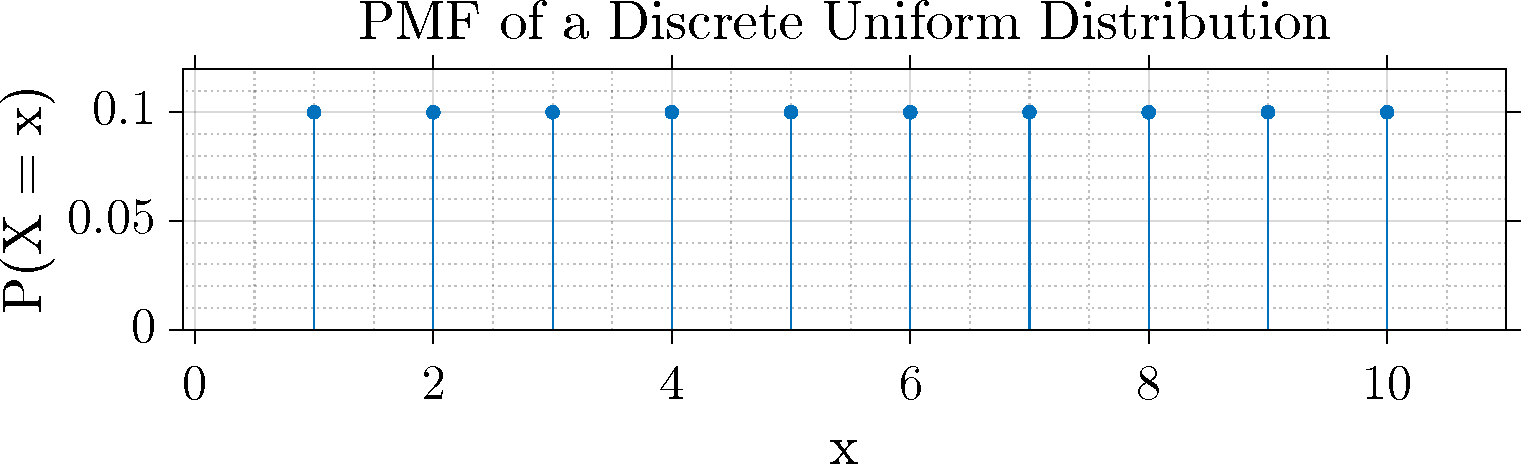
\includegraphics[width=.9\textwidth]{figures/DiscreteUniform.pdf}
    \end{center}
    \end{frame}
    
    %------------------------------------------------
    
    \begin{frame}[containsverbatim]{Hypergeometric Distribution}
    
        \begin{tblock}{2. Hypergeometric}
        \begin{multiequation}
                    P(X = x|M, N, K) & = \cfrac{ {M \choose x} {N-M \choose K-x} }{{N \choose K}}\\
                    \Ebb(X) & = \cfrac{KM}{N}\\
                    var(X) & = K \cfrac{M}{N} \cfrac{(N-M)(M-K)}{N(N-1)}
        \end{multiequation}
        The following problem exhibits Hypergeometric distribution: there is a large urn filled with $N$ balls, $M$ red, and $N-M$ green balls. Draw $K$ balls at random without replacement.
        \end{tblock}

    \end{frame}
    
    \begin{frame}[containsverbatim]{Hypergeometric Distribution}

    
            \begin{center}
    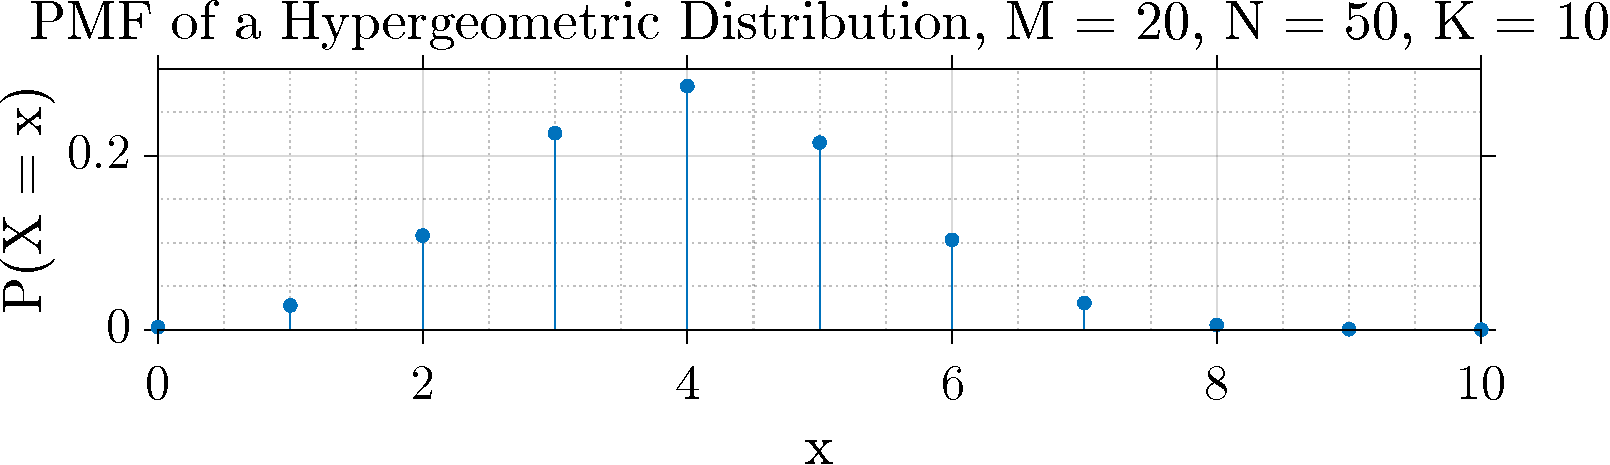
\includegraphics[width=.9\textwidth]{figures/Hypergeometric.pdf}
    \end{center}
    
    \end{frame}
    
    %------------------------------------------------
    \begin{frame}[containsverbatim]{Binomial Distribution}
    
    
        \begin{tblock}{3. Binomial}
            Repeat a random experiment $n$ times that satisfies the following conditions
            \begin{enumerate}
                \item Only two possible outcomes: success and failure.
                \item The probability of success $p$ is the same for each trial.
                \item The experiments are independent of each other.
                \item $X = $ the number of total number of success in $n$ trials.
            \end{enumerate}
        We call these Bernoulli trials. We can then write as $X \sim Bin(n, p)$ with pmf: 
        \begin{multiequation}
                    P(X = x) & ={n \choose x} p^x ( 1 - p)^{n-x}, \quad x = 0, 1, \cdots n\\
                    \Ebb(X) & = np\\
                    var(X) & = np(1-p)
        \end{multiequation}
        \end{tblock}
    
    \end{frame}
    
    \begin{frame}[containsverbatim]{Binomial Distribution}


     \begin{center}
    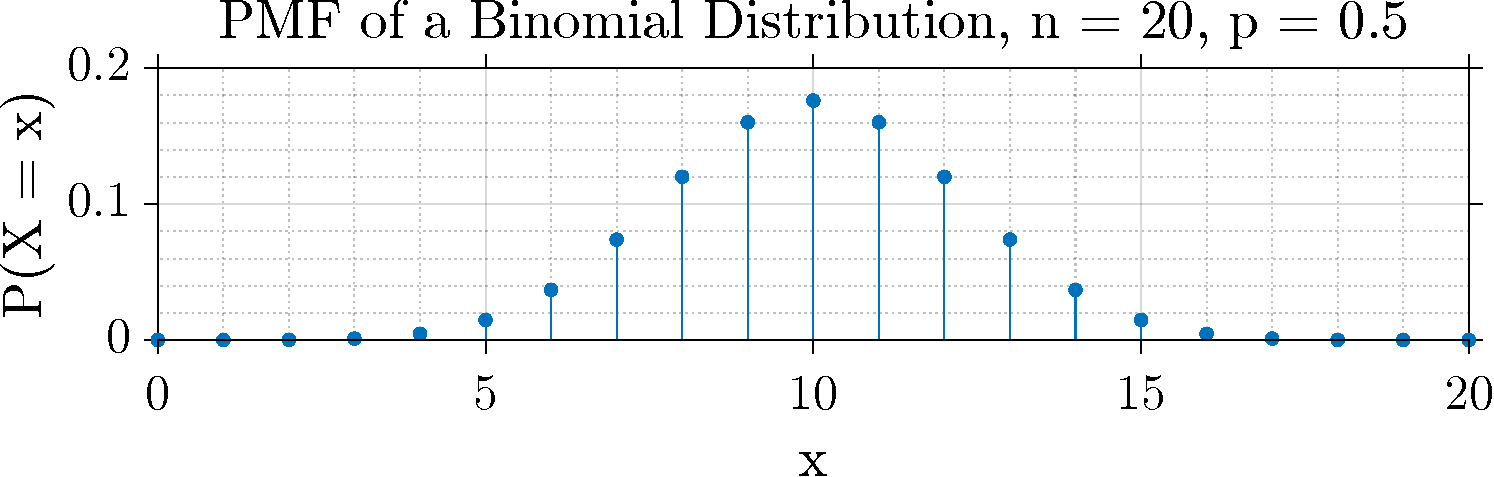
\includegraphics[width=.9\textwidth]{figures/Binomial.pdf}
    \end{center}
    
    
    \end{frame}
    
    %------------------------------------------------
    
    \begin{frame}[containsverbatim]{Poisson Distribution}
        \begin{tblock}{4. Poisson}
            The random variable X takes non-negative integer values such that
            \begin{multiequation}
                    P(X = x) & = \cfrac{e^{-\lambda}\lambda^x}{x!}, \quad x = 0, 1, \cdots\\
                    \Ebb(X) & = \lambda\\
                    var(X) & = \lambda
            \end{multiequation}
        \end{tblock}
    \end{frame}
    
    \begin{frame}[containsverbatim]{Poisson Distribution}

        Poisson distribution is often used for describing the number of occurrences of a certain event in a very large number of observations, the probability for the event to occur in each observation being very small. Some examples: (i) Nuclear decay of atoms; (ii) Mutation of DNA; (iii) Photon counting by a photodetector.

    \end{frame}
    
    \begin{frame}[containsverbatim]{Poisson Distribution}

    
         \begin{center}
    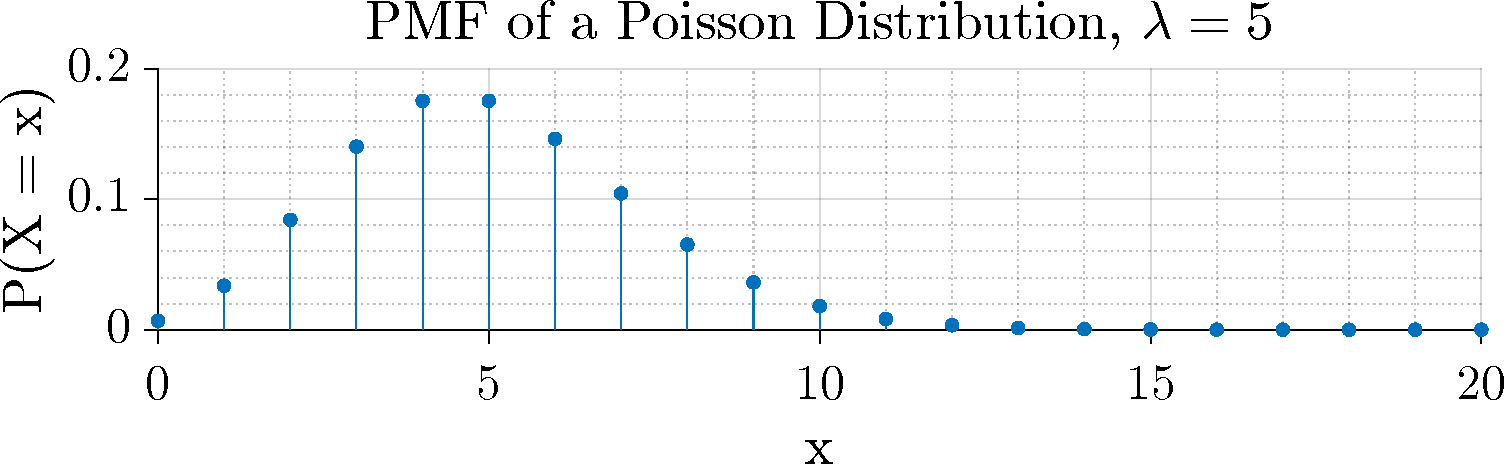
\includegraphics[width=.9\textwidth]{figures/Poisson.pdf}
    \end{center}
    
    \end{frame}
    
    %------------------------------------------------
    \subsection{Common Families of Distribution: Continuous Distribution}
    %------------------------------------------------
    
    
    \begin{frame}
    \subsectionpage
\end{frame}
    %------------------------------------------------
    
    \begin{frame}[containsverbatim]{Continuous Uniform Distribution}
    \begin{tblock}{5. Continuous Uniform}
    We say $X\sim Unif(a, b)$ if it has PDF 
        \begin{multiequation}
    f(x | a, b) & = \cfrac{1}{b - a}, \quad a < x < b\\
     \Ebb(X) & =\cfrac{1}{a+b}\\
                    var(X) & = \cfrac{1}{12}(b-a)^2
                 \end{multiequation}
    \end{tblock}
\end{frame}
\begin{frame}[containsverbatim]{Continuous Uniform Distribution}

        \begin{center}
    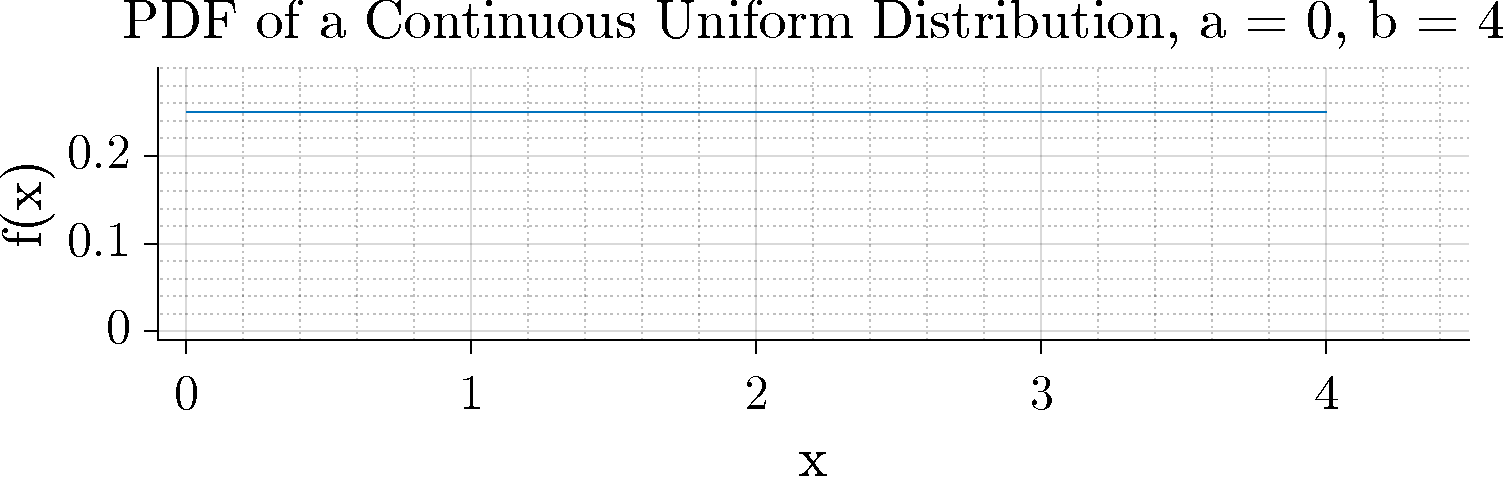
\includegraphics[width=.9\textwidth]{figures/ContinuousUniform.pdf}
    \end{center}
    
    \end{frame}
    
    %------------------------------------------------
    
    \begin{frame}[allowframebreaks, containsverbatim]{Exponential Family Distribution}
    \begin{tblock}{6. Exponential Family}
    We say $X\sim Exp(\beta)$ if it has PDF 
        \begin{multiequation}
    f(x | \beta) & = \cfrac{1}{\beta}e^{-x/\beta}, \quad  x  > 0\\
     \Ebb(X) & =\beta\\
                    var(X) & = \beta^2
                 \end{multiequation}
    \end{tblock}

\end{frame}
\begin{frame}[containsverbatim]{Exponential Family Distribution}

    
        \begin{center}
    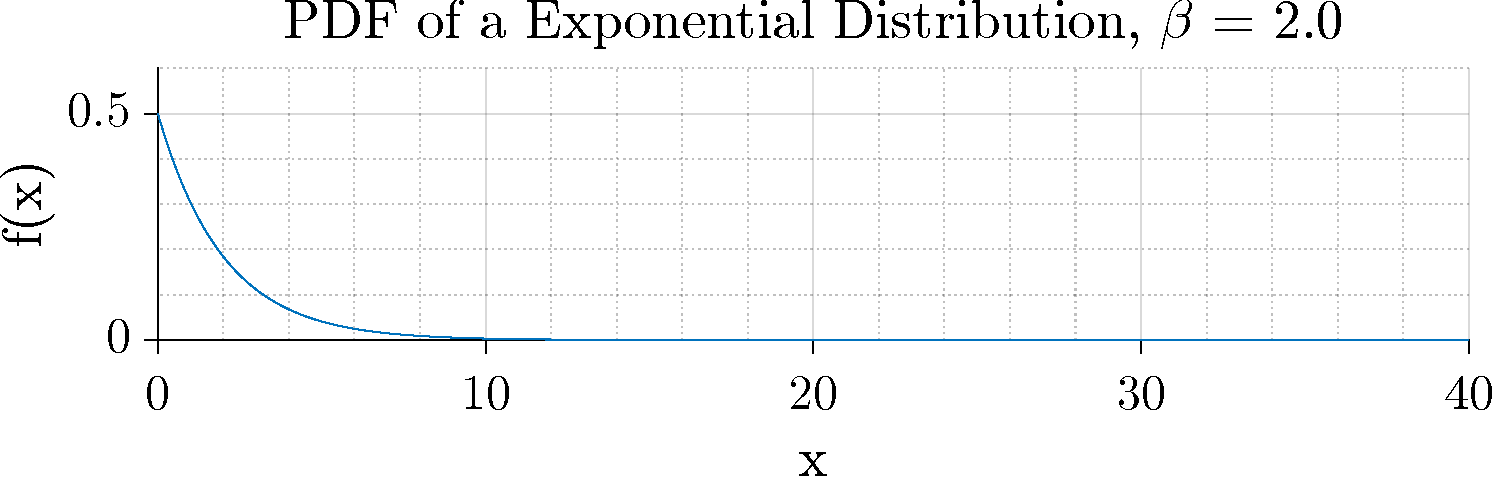
\includegraphics[width=.9\textwidth]{figures/Exponential.pdf}
    \end{center}
    
    \end{frame}
    
    %------------------------------------------------
    
    \begin{frame}[containsverbatim]{Gamma Family Distribution}
    \begin{tblock}{6. Gamma Family}
    For a random variable $X$, Gamma distribution is characterized by two parameters: $\alpha$ and $\beta$. Its PDF is given by
    \begin{equation}
        f(x | \alpha, \beta) = \cfrac{1}{\beta^\alpha \Gamma(\alpha)} e^{-x/\beta}x^{\alpha - 1}
    \end{equation}
    
    where gamma function $ \Gamma(\alpha)$ is given by
    $     \Gamma(\alpha) = \int_0^\infty e^{-x}x^{\alpha -1 }dx
    $.
    In the gamma distribution, $\alpha$ is a shape parameter that defines the peakedness of the distribution while $\beta$ is a scale parameter that influences the spread of the distribution.
    The mean of the gamma distribution, $\Ebb(X) =\alpha\beta$ while the variance $var(X) = \alpha\beta^2$.
    \end{tblock}
\end{frame}
    
%------------------------------------------------

\begin{frame}[containsverbatim]{Gamma Family Distribution}
    
     \begin{center}
    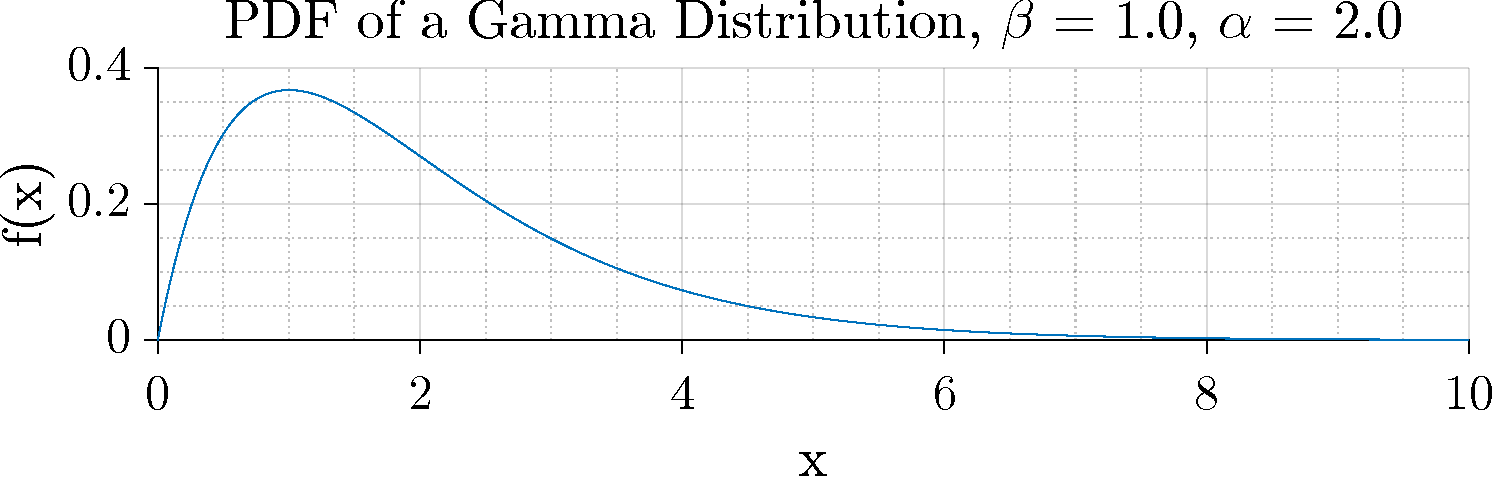
\includegraphics[width=.9\textwidth]{figures/Gamma.pdf}
    \end{center}
    
    \end{frame}
    
    %------------------------------------------------
    
    \begin{frame}[allowframebreaks]{Weibull Distribution}
    
    \begin{tblock}{7. Weibull}
        If we have a random variable $X\sim Exp(\beta)$, and another random variable $Y \sim X^{1/\gamma}$, then in this case the $Y$ follows a distribution called as Weibull distribution. The PDF of Weibull distribution is given by 
        \begin{equation}
            f(y|\beta, \gamma) = \cfrac{\gamma}{\beta}y^{\gamma - 1}e^{-y^\gamma/\beta}, \quad y > 0
        \end{equation}
    \end{tblock}

        
\end{frame}
    
%------------------------------------------------

\begin{frame}[allowframebreaks]{Weibull Distribution}

    
    For the Weibull distribution, the mean and variance are given by
    \begin{multiequation}
        \Ebb(Y) & = \beta^{1/\gamma}\Gamma(1 + \cfrac{1}{\gamma} )\\
        var(Y) & = \beta^{2/\gamma}\bigg[\Gamma(1 +\tfrac{2}{\gamma}) - \bigg(\Gamma(1 +\tfrac{2}{\gamma})\bigg)^2 \bigg]
    \end{multiequation}

\end{frame}
    
%------------------------------------------------

\begin{frame}[allowframebreaks]{Weibull Distribution}
    
    \begin{facts}{Remark}
       The difference between the Weibull and Gamma distributions is that in the Gamma distribution, $y$ has a linear term in the exponential while in the Weibull distribution, there is $y$ to the power $\gamma$.
        
    \end{facts}
    
\end{frame}
    
%------------------------------------------------

\begin{frame}[allowframebreaks]{Weibull Distribution}

     \begin{center}
    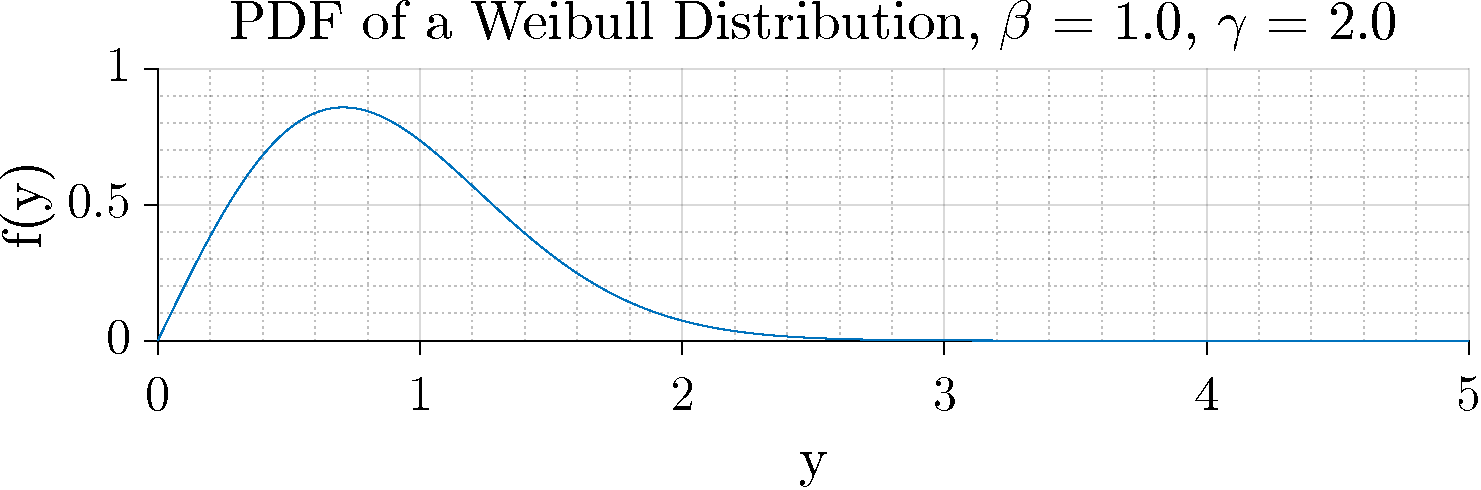
\includegraphics[width=.9\textwidth]{figures/Weibull.pdf}
    \end{center}
    
    \end{frame}
    
    %------------------------------------------------
    
    \begin{frame}[allowframebreaks]{Normal Distribution/Gaussian Distribution}
        \begin{tblock}{8. Gaussian}
            Gaussian distribution is the most common distribution everyone is familiar with. For a random variable $X$ following a Gaussian distribution, we write $X\sim N(\mu, \sigma^2)$. Its PDF is given by
            \begin{equation}
                f(x | \mu, \sigma) = \cfrac{1}{\sqrt{2\pi}\sigma} e ^{- \tfrac{(x-\mu)^2}{2\sigma^2}}
            \end{equation}
        \end{tblock}
        Its expectations and variance are given by $\Ebb(X) = \mu$, and $var(X) = \sigma^2$ respectively. A standard normal distribution has a mean of 0 and a variance of 1 denoted as $X\sim N(0,1)$.
        \end{frame}
    
    %------------------------------------------------
    
    \begin{frame}[allowframebreaks]{Normal Distribution/Gaussian Distribution}

             \begin{center}
    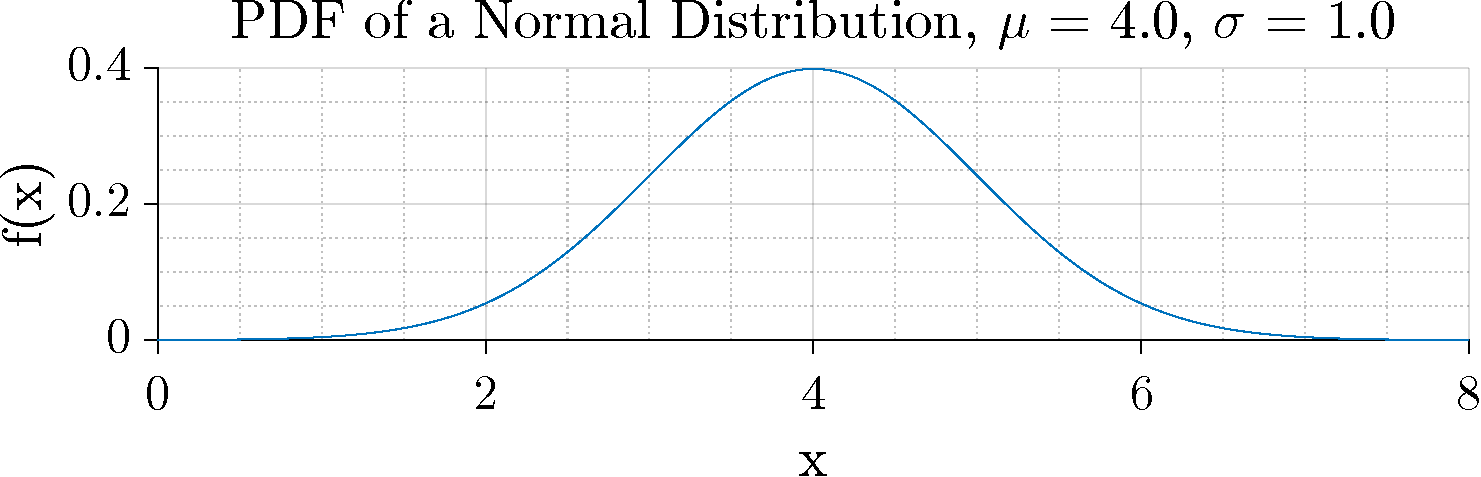
\includegraphics[width=.9\textwidth]{figures/Normal.pdf}
    \end{center}
    
    
    \end{frame}
    
    %------------------------------------------------
    
    \begin{frame}[allowframebreaks]{Laplace Distribution}
        \begin{tblock}{9. Laplace}
            A random variable X following the Laplace distribution, also known as the double exponential distribution has the following PDF:
        \begin{equation}
            f(x|\mu, \sigma) = \cfrac{1}{2\sigma}e^{-|x-\mu|/\sigma}, \quad -\infty < x < \infty
        \end{equation}
    
        Its mean and variance are given by $\Ebb(X) = \mu$, $var(X) = 2\sigma^2$ respectively.
        
        \end{tblock}
        \end{frame}
    
    %------------------------------------------------
    
    \begin{frame}[allowframebreaks]{Laplace Distribution}
      \begin{center}
    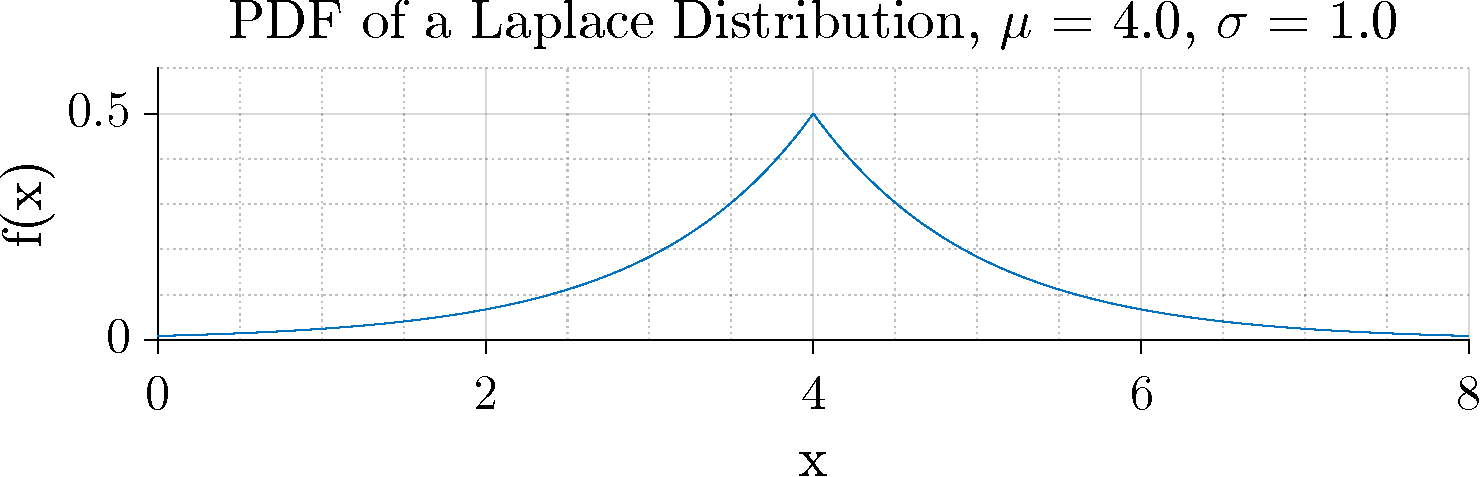
\includegraphics[width=.9\textwidth]{figures/Laplace.pdf}
    \end{center}
        
    \end{frame}
    
    %------------------------------------------------
    \subsection{Synthetic Data Generation from Common Families of Distribution}
    %------------------------------------------------
    
    
    \begin{frame}
    \subsectionpage
\end{frame}
    
    %------------------------------------------------
    
    \begin{frame}[containsverbatim]{Generating Data from Discrete Distribution}
    
    \begin{gradblock}{\texttt{scipy.stats.rv\_discrete}}
        Synthetic datasets from distributions discussed above can be generated using \texttt{scipy.stats.rv\_discrete}. Below is the code snippet that requires Python 3.8 or above followed by a stem plot showing the PMF of each distribution.
    \end{gradblock}
\end{frame}
    
%------------------------------------------------

\begin{frame}[containsverbatim]{Generating Data from Discrete Distribution}

    \begin{facts}
        \texttt{rv\_discrete} is a base class to construct specific distribution classes and instances for discrete random variables. It can also be used to construct an arbitrary distribution defined by a list of support points and corresponding probabilities.
    
    It allows you to sample a random number of that particular distribution you are specifying, thereby generating synthetic datasets that follow the given distribution.
    \end{facts}
    
\end{frame}
    
%------------------------------------------------

\begin{frame}[containsverbatim]{Generating Data from Hypergeometric Distribution}

    \begin{minted}
    [
    framesep=1mm,
    baselinestretch=1.2,
    fontsize=\footnotesize
    ]
    {python}
    # hypergeometric
    N = 100
    M = 50
    K = 10
    x2k = np.arange(min(M,K))
    y2k = np.zeros(min(M,K))
    for i, x in enumerate(x2k):
        y2k[i] = (math.comb(M, x)*math.comb(N-M, K-x))/math.comb(N, K)
    # because of numerical round off and how many samples 
    # we choose, sum of y2k is less than 1. So just normalize it
    y2k =y2k/sum(y2k)
    
    # Create a probability Mass Function
    pmf2 = rv_discrete(name='hypergeometric', values=(x2k, y2k))
    \end{minted}

    
    \end{frame}
    
    %------------------------------------------------
    
    \begin{frame}[containsverbatim]{Plotting Probability Mass Functions}
 
    \begin{minted}
    [
    framesep=1mm,
    baselinestretch=1.2,
    fontsize=\tiny
    ]
    {python}
    import matplotlib.pyplot as plt
    fig, ax = plt.subplots(2, 1)
    ax=np.ravel(ax)
    
    ax[0].plot(x1k, pmf1.pmf(x1k), 'o', ms=6, mec='#2F9C95', markerfacecolor="#2F9C95")
    ax[0].vlines(x1k, 0, pmf1.pmf(x1k), colors='#2F9C95', lw=1)
    ax[0].set_title('Uniform Discrete')
    
    ax[1].plot(x2k, pmf2.pmf(x2k), 'o', ms=6, mec='#2F9C95', markerfacecolor="#2F9C95")
    ax[1].vlines(x2k, 0, pmf2.pmf(x2k), colors='#2F9C95', lw=1)
    ax[1].set_title('Hypergeometric')
    
    plt.tight_layout()
    plt.show()
    \end{minted}

    \end{frame}
    
    \begin{frame}[containsverbatim]{Plotting Probability Mass Functions}
    \begin{center}
        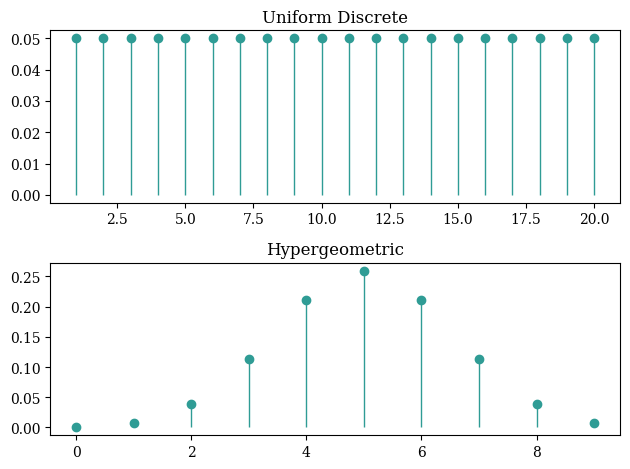
\includegraphics[height=.6\textheight]{figures/PMFs.png}
    
    \end{center}
    \end{frame}
    
    %------------------------------------------------
    
    \begin{frame}[containsverbatim]{Generating Data from Continuous Distribution}
    \begin{gradblock}{\texttt{scipy.stats.rv\_continuous}}
        Synthetic datasets from continuous distributions discussed in the lecture can be generated using \texttt{scipy.stats.rv\_continuous}. Below is the code snippet that requires Python 3.8. Code is followed by a histogram plot of the probability density function of some distributions discussed here.
    \end{gradblock}
\end{frame}
    
%------------------------------------------------

\begin{frame}[containsverbatim]{Generating Data from Exponential Distribution}

    \begin{minted}
    [
    framesep=1mm,
    baselinestretch=1.2,
    fontsize=\footnotesize
    ]
    {python}
    class Exponential(rv_continuous):
        "Exponential"
        def __init__(self, beta, **kwargs):
            super().__init__(**kwargs)
            self.beta = beta
        def _pdf(self, x):
            if(x <=0):
                return 0
            y = (1.0/self.beta)*np.exp(-x/self.beta)
            return y
    P2 = Exponential(name='Exponential', beta = 2.0)
    # Sample 1000 numbers
    B2 = P2.rvs(size = 1000)
    \end{minted}

\end{frame}
    
%------------------------------------------------

\begin{frame}[containsverbatim]{Generating Data from Gamma Distribution}


    
    \begin{minted}
    [
    framesep=1mm,
    baselinestretch=1.2,
    fontsize=\footnotesize
    ]
    {python}
    class Gamma(rv_continuous):
        "Gamma"
        def __init__(self, alpha, beta, **kwargs):
            super().__init__(**kwargs)
            self.alpha = alpha
            self.beta = beta
        def _pdf(self, x):
            if(x <=0):
                return 0
            y = (1.0/((self.beta**self.alpha)*gamma(self.alpha)))*
                            np.exp(-x/self.beta)*(x**(self.alpha-1))
            return y
    P3 = Gamma(name='Gamma', alpha = 1, beta = 0.5)
    B3 = P3.rvs(size = 1000)
    \end{minted}
    \end{frame}
    
    %------------------------------------------------
    
    \begin{frame}[containsverbatim]{Plotting Probability Density Functions}
    \begin{tblock}{Plotting PDFs}
    \begin{minted}
    [
    framesep=1mm,
    baselinestretch=1.2,
    fontsize=\tiny
    ]
    {python}
    fig, ax = plt.subplots(2, 1)
    ax=np.ravel(ax)
    a= s.histplot(B2, ax = ax[0], stat = 'density', kde=True)
    s.kdeplot(B2, color='crimson', ax=a)
    ax[0].set_xlim([0, 15])
    ax[0].set_xlabel('x',  fontsize = 20)
    ax[0].set_ylabel('f(x)', fontsize =20)
    ax[0].set_title('Exponential', fontsize =20)
    a = s.histplot(B3, ax = ax[1], stat = 'density', kde=True)
    s.kdeplot(B3, color='crimson', ax=a)
    ax[1].set_xlim([0, 15])
    ax[1].set_xlabel('x',  fontsize = 20)
    ax[1].set_ylabel('f(x)', fontsize =20)
    ax[1].set_title('Gamma', fontsize =20)
    plt.tight_layout()
    \end{minted}
    \end{tblock}
    \end{frame}
    
    \begin{frame}[containsverbatim]{Plotting Probability Density Functions}
    \begin{center}
        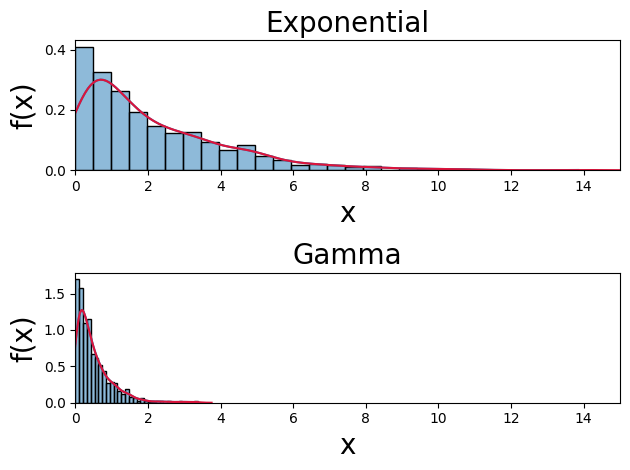
\includegraphics[height=.6\textheight]{figures/PDFs.png}
    
    \end{center}
    \end{frame}
    
    %------------------------------------------------
    
    \begin{frame}[containsverbatim]{Python Notebook for Synthetic Data Generation}
    \begin{center}
    \small
    { \color{Red}{\url{https://github.com/rahulbhadani/CPE486586_FA25/blob/main/Code/CPE486586_Ch04_SyntheticDataGeneration.ipynb}}}
    
    \end{center}
    \end{frame}
    
    \begin{frame}{References}

        \begin{columns}
            \column{0.5\linewidth}
            \begin{center}
        
\includegraphics[height=.6\textheight]{figures/stat_computing.jpg}
        
        \vspace{1.5pt}

        Chapter 2.
    \end{center}
    \column{0.5\linewidth}
            \begin{center}
        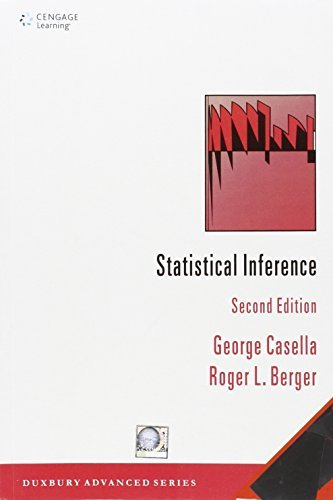
\includegraphics[height=.6\textheight]{figures/Statistical_inference.jpg}
    \end{center}
        \end{columns}
        
    \end{frame}
    %------------------------------------------------
    
    \begin{frame}
        \Huge{\centerline{\color{MediumBlue}\textbf{The End}}}
    \end{frame}


\end{document}